% Editable source restored from Novichkov_IAD_DirectLiNGAM (1).tex.
% Updated to the supplied Novichkov_IAD_DirectLiNGAM (6) (1).pdf (14 pages).
% The supplied slides.pdf is preserved byte-for-byte, not replaced by a rebuild.
% Figures were extracted from that PDF; text, formulas and diagrams remain editable.
% Build from this directory with a full TeX Live / MiKTeX installation:
%   pdflatex -interaction=nonstopmode -halt-on-error slides.tex
%   pdflatex -interaction=nonstopmode -halt-on-error slides.tex
% Requires Beamer, Russian Babel, T2A / CM-Super, TikZ, pgfplots,
% csquotes, booktabs and appendixnumberbeamer.

\documentclass[aspectratio=169]{beamer}

% Based on kisnikser/intsystems-slides/report/main.tex.
\usepackage[10pt]{type1ec}
\usepackage[T1,T2A]{fontenc}
% Scalable Computer Modern Cyrillic, also suitable for minimal CM-Super installs.
\DeclareFontShape{T2A}{cmss}{m}{n}{<->lass1000}{}
\DeclareFontShape{T2A}{cmss}{m}{sl}{<->lasi1000}{}
\DeclareFontShape{T2A}{cmss}{m}{it}{<->lasi1000}{}
\DeclareFontShape{T2A}{cmss}{bx}{n}{<->lasx1000}{}
\DeclareFontShape{T2A}{cmss}{bx}{it}{<->laso1000}{}
\DeclareFontShape{T2A}{cmss}{bx}{sl}{<->laso1000}{}
\usepackage[utf8]{inputenc}
\usepackage[main=russian,english]{babel}
\usepackage{cmap}
\usepackage{tikz}
\usetikzlibrary{arrows.meta,positioning,calc}
\usepackage{array,multicol,booktabs,csquotes}
\usepackage{amssymb,amsfonts,amsmath}
\usepackage{pgfplots}
\pgfplotsset{compat=1.18}
\usepackage{appendixnumberbeamer}
\graphicspath{{figures/}{slides/figures/}}
\pdfmapfile{+cm-super-t2a.map}

\usecolortheme{beaver}
\usefonttheme[onlymath]{serif}
\setbeamertemplate{navigation symbols}{}
\setbeamertemplate{footline}[frame number]
\setbeamertemplate{blocks}[rounded=true,shadow=true]
\setbeamersize{text margin left=0.5cm,text margin right=0.5cm}
\setbeamerfont{author}{size=\normalsize}
\setbeamerfont{institute}{size=\normalsize}
\setbeamerfont{date}{size=\normalsize}
\setbeamertemplate{enumerate item}{\insertenumlabel)}
\setbeamertemplate{enumerate subitem}{\insertenumlabel)}
\setbeamertemplate{enumerate subsubitem}{\insertenumlabel)}
\setlength{\tabcolsep}{6pt}
\newcommand{\src}[1]{\par\vspace{0.10cm}{\fontsize{6.5}{7.5}\selectfont\color{gray}#1\par}}
\newcommand{\lead}[1]{{\usebeamercolor[fg]{block title}\textbf{#1}}}
\newcommand{\given}{\;|\;}

\title{Классификация многомерных временных рядов}
\subtitle{Графы зависимостей как признаки активности}
\author{Новичков Григорий}
\date{Ноябрь 2026}


% Original notebook edge grid; native labels remain readable on the slide.
\newcommand{\timegraph}[1]{%
    \begin{tikzpicture}[x=1cm,y=1cm]
        \node[anchor=south west,inner sep=0] at (0,0) {\includegraphics[width=5.15cm]{#1}};
        \foreach \xx/\tt in {0.371/{t-2},2.538/{t-1},4.697/{t}} {
            \node[font=\small] at (\xx,5.23) {$\tt$};
        }
        \foreach \yy/\nn in {4.697/{back\_x},3.824/{back\_y},2.951/{back\_z},2.077/{thigh\_x},1.195/{thigh\_y},0.321/{thigh\_z}} {
            \node[anchor=east,font=\footnotesize] at (-0.06,\yy) {\nn};
        }
    \end{tikzpicture}%
}

\begin{document}

\begin{frame}
    \thispagestyle{empty}
    \maketitle
\end{frame}

\begin{frame}{Постановка задачи классификации}
    \small
    \begin{block}{Дано}
        $X\in\mathbb R^{500\times6}$ --- сигналы двух трёхосевых
        акселерометров (прибор измеряющий ускорения предмета в трех направлениях $a_x$, $a_y$, $a_z$). Каждому объекту соотвествует $y\in\{\text{ходьба},\text{бег}\}$.
    \end{block}
    \begin{block}{Найти}
        По размеченным окнам $\{(X_i,y_i)\}_{i=1}^{n}$ построить правило
        $\widehat y=f(X)$ для окна нового участника.
    \end{block}
    \begin{block}{Проверяемая гипотеза}
        Каждый процесс (ходьба, бег) имеет свой уникальный причинно-следственный граф. С помощью которого мы можем хорошо классифицировать данные.
    \end{block}
    \begin{block}{Метод}
        Воспользуемся алгоритмами DIRECTLINGAM и другими (DYNOTEARS, PCMCIA+) для восстановления причинно-следственного графа каждого процесса по его временным рядам.
    \end{block}
\end{frame}

\begin{frame}[t]{Что такое причинно-следственный граф?}
    Вершины графа --- переменные. Пусть $V=f_V(U,Z,\varepsilon_V)$
    --- уравнение для $V$, где $Z$ --- остальные входы, а $\varepsilon_V$ --- шум.
    \[
        \boxed{
            U\to V
            \quad\Longleftrightarrow\quad
            \exists\,u\ne u',\,z,\,e\ \text{такие, что}\
            f_V(u,z,e)\ne f_V(u',z,e).
        }
    \]
    Проводим стрелку от $U$ к $V$, если изменение $U$ при тех же
    $Z$ и $\varepsilon_V$ может изменить $V$.

    \medskip
    \begin{columns}[c,onlytextwidth]
        \begin{column}{0.53\textwidth}
            \lead{Пример.} Предполагаем $a,b,c\ne0$.
            \[
                \begin{aligned}
                    X_t &= aX_{t-1}+\varepsilon_t^X,\\
                    Y_t &= bX_{t-1}+cY_{t-1}+\varepsilon_t^Y.
                \end{aligned}
            \]
        \end{column}
        \begin{column}{0.43\textwidth}
            \centering
            \begin{tikzpicture}[>=Stealth, every node/.style={font=\normalsize}]
                \node (xm) at (0,1.7) {$X_{t-1}$};
                \node (xt) at (3.1,1.7) {$X_t$};
                \node (ym) at (0,0) {$Y_{t-1}$};
                \node (yt) at (3.1,0) {$Y_t$};
                \draw[->,thick] (xm) -- node[above] {$a$} (xt);
                \draw[->,thick] (ym) -- node[above] {$c$} (yt);
                \draw[->,thick,red!65!black] (xm) -- node[above] {$b$} (yt);
            \end{tikzpicture}
        \end{column}
    \end{columns}

    \par\vfill
    \small Далее рассматриваем графы для нескольких временных рядов с некоторым фиксированным .
    Вершина $X_t$ обозначает переменную $X$ в момент $t$.
\end{frame}

\begin{frame}{Модель LiNGAM}
    \[
        X_i=\sum_{j\ne i} b_{ij}X_j+\varepsilon_i.
    \]
    $X_i$ складывается из линейной комбинации других переменных
    и некоторого негауссовского шума $\varepsilon_i$.
    \par\smallskip
    В матрице $B=(b_{ij})$ ненулевой $b_{ij}$ задаёт ребро $X_j\to X_i$.
    \par\medskip
    \lead{Основные предположения}
    \begin{itemize}
        \item Граф ацикличен.
        \item Скрытых общих причин нет.
        \item Шумы взаимно независимы, $0<\operatorname{Var}(\varepsilon_i)<\infty$.
    \end{itemize}
\end{frame}

\begin{frame}[t]{Алгоритм DirectLiNGAM}
    \small
    \setlength{\abovedisplayskip}{3pt}
    \setlength{\belowdisplayskip}{3pt}
    \setlength{\abovedisplayshortskip}{2pt}
    \setlength{\belowdisplayshortskip}{2pt}
    \lead{0. Центрирование.} Для всех $i$ вычитаем среднее,
    $X_i\leftarrow X_i-\mathbb E[X_i]$.
    \par\smallskip
    \lead{1. Топологическая сортировка.} Для каждой пары $i\ne j$
    регрессируем $X_i$ на $X_j$. $I$ --- взаимная информация.
    \[
        \beta_{ij}=\frac{\operatorname{Cov}(X_i,X_j)}{\operatorname{Var}(X_j)},\qquad
        r_i^{(j)}=X_i-\beta_{ij}X_j,\qquad
        S(j)=\textstyle\sum_{i\ne j} I\bigl(X_j;r_i^{(j)}\bigr).
    \]
    \lead{Критерий корня.}\quad
    $\boxed{S(j)=0\ \Longleftrightarrow\ X_j\text{ --- корень}}$
    \par\smallskip
    \lead{1.1. Корень.}\quad
    $X_j=\varepsilon_j,\quad
    r_i^{(j)}=\sum_{k\ne j}d_{ik}\varepsilon_k
    \quad\Longrightarrow I\bigl(X_j;r_i^{(j)}\bigr)=0\quad(\forall\,i\ne j)$
    \par\smallskip
    \lead{1.2. Есть родители.}\quad
    $X_j=\varepsilon_j+\ldots,\quad
    r_i^{(j)}=-\beta_{ij}\varepsilon_j+\ldots
    \ \Longrightarrow I\bigl(X_j;r_i^{(j)}\bigr)>0\quad(\exists\,i\ne j)$
    \par\smallskip
    Шум корня независим от остальных. Во второй строке $i$ --- родитель
    с $\beta_{ij}\ne0$. Общий негауссовский $\varepsilon_j$ даёт зависимость
    по Дармуа--Скитовичу.
    \par\smallskip
    Берём узел с минимальной оценкой $S$, записываем в порядок и удаляем.
    Остатки снова образуют LiNGAM, повторяем поиск на них.
    \par\smallskip
    \lead{2. Рёбра.} На исходных данных регрессируем $X_i$ на все узлы до него
    в найденном порядке. Ребро $X_j\to X_i$ при $b_{ij}\ne0$.
    \src{В статье $I$ оценивают ядерной мерой. Shimizu et al. (2011), JMLR 12, \S\,3.2--3.3.}
\end{frame}

\begin{frame}[t]{Пример DirectLiNGAM на трёх переменных}
    \small
    \setlength{\abovedisplayskip}{4pt}
    \setlength{\belowdisplayskip}{4pt}
    \setlength{\abovedisplayshortskip}{3pt}
    \setlength{\belowdisplayshortskip}{3pt}
    \tikzset{
        lingam node/.style={circle,draw=black!55,fill=black!5,
            minimum size=6.4mm,inner sep=0pt},
        lingam root/.style={lingam node,very thick,draw=blue!65!black,fill=blue!13}
    }

    Шумы независимы и негауссовские, $\mathbb E[\varepsilon_i]=0$, $\operatorname{Var}(\varepsilon_i)=1$.
    \[
        Z=\varepsilon_Z,\qquad Y=Z+\varepsilon_Y,\qquad
        X=2Y+Z+\varepsilon_X.
    \]
    \begin{columns}[T,onlytextwidth]
        \begin{column}{0.48\textwidth}
            \centering\lead{1. Проверяем $Z$}\par\smallskip
            \begin{tikzpicture}[>=Stealth]
                \path[use as bounding box] (-0.38,-0.40) rectangle (3.38,1.06);
                \node[lingam root] (z) at (0,0) {$Z$};
                \node[lingam node] (y) at (1.5,0.69) {$Y$};
                \node[lingam node] (x) at (3,0) {$X$};
                \draw[->,thick,blue!75!black] (z) -- node[above left] {$1$} (y);
                \draw[->,thick,blue!75!black] (z) -- node[below] {$1$} (x);
                \draw[->,thick] (y) -- node[above right] {$2$} (x);
            \end{tikzpicture}\par
            {\color{green!55!black}$S(Z)=0$}\quad {\color{red}$S(X),S(Y)>0$}\par\smallskip
            \raggedright
            \[
                \begin{aligned}
                    Y'&=Y-Z=\varepsilon_Y,\\
                    X'&=X-3Z=2\varepsilon_Y+\varepsilon_X.
                \end{aligned}
            \]
            Оба остатка независимы от $Z$. У $X$ и $Y$ есть родители. Выбираем $Z$.
        \end{column}

        \begin{column}{0.48\textwidth}
            \centering\lead{2. Повторяем на остатках}\par\smallskip
            \begin{tikzpicture}[>=Stealth]
                \path[use as bounding box] (-0.38,-0.40) rectangle (3.38,1.06);
                \node[lingam root] (yr) at (0.6,0.38) {$Y'$};
                \node[lingam node] (xr) at (2.4,0.38) {$X'$};
                \draw[->,thick,blue!75!black] (yr) -- node[above] {$2$} (xr);
            \end{tikzpicture}\par
            {\color{green!55!black}$S(Y^{\prime})=0$}\quad {\color{red}$S(X^{\prime})>0$}\par\smallskip
            \raggedright
            \[
                \begin{aligned}
                    r_{X'}^{(Y')}&=X'-2Y'=\varepsilon_X,\\
                    r_{Y'}^{(X')}&=Y'-\tfrac25X'=\tfrac15(\varepsilon_Y-2\varepsilon_X).
                \end{aligned}
            \]
            Первый остаток независим от $Y'$. Второй и $X'$ содержат $\varepsilon_X$. Выбираем $Y'$.
        \end{column}
    \end{columns}

    \par\smallskip
    \lead{Итог.} Порядок $(Z,Y,X)$. МНК даёт веса $1$ для $Z\to Y$ и
    $Z\to X$, вес $2$ для $Y\to X$.
\end{frame}

\begin{frame}{Синтетика:}
    \small Граф переменных $x$,$y$,$z$ с лагами $t-2$, $t-1$, $t$.
    \vspace{0.10cm}
    \begin{columns}[T]
        \begin{column}{0.49\textwidth}
            \centering\lead{Известный граф}\par\smallskip
            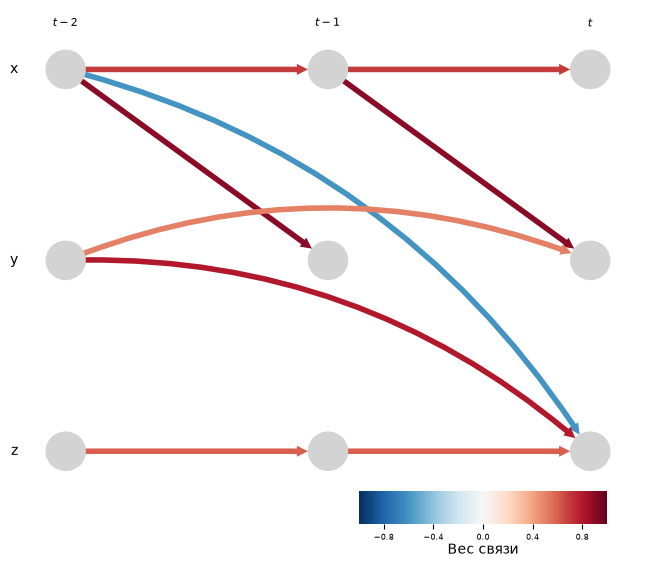
\includegraphics[height=4.45cm,width=\linewidth,keepaspectratio]{synthetic_truth.png}
        \end{column}
        \begin{column}{0.49\textwidth}
            \centering\lead{DirectLiNGAM}\par\smallskip
            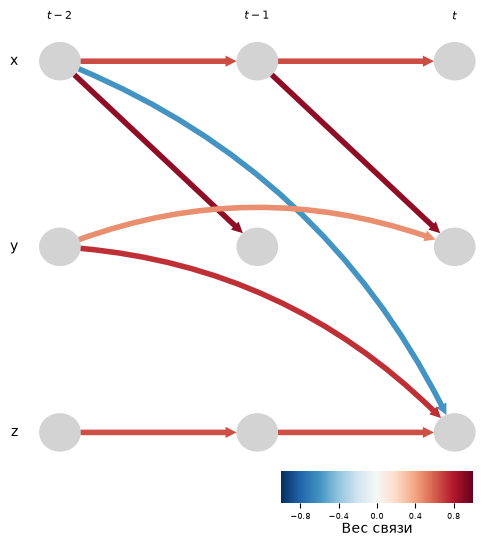
\includegraphics[height=4.45cm,width=\linewidth,keepaspectratio]{synthetic_var_window500.png}
        \end{column}
    \end{columns}
    \setlength{\abovedisplayskip}{4pt}
    \setlength{\belowdisplayskip}{4pt}
    \setlength{\abovedisplayshortskip}{4pt}
    \setlength{\belowdisplayshortskip}{4pt}
    \[
        x_t=0.7x_{t-1}+\varepsilon^x_t,\quad
        y_t=0.9x_{t-1}+0.5y_{t-2}+\varepsilon^y_t,\quad
        z_t=0.6z_{t-1}+0.8y_{t-2}-0.6x_{t-2}+\varepsilon^z_t.
    \]
    Шумы негауссовские и независимы. На этом окне метод восстановил все шесть типов рёбер.
\end{frame}

\begin{frame}{HARTH: разведочный анализ четырёх активностей}
    \centering
    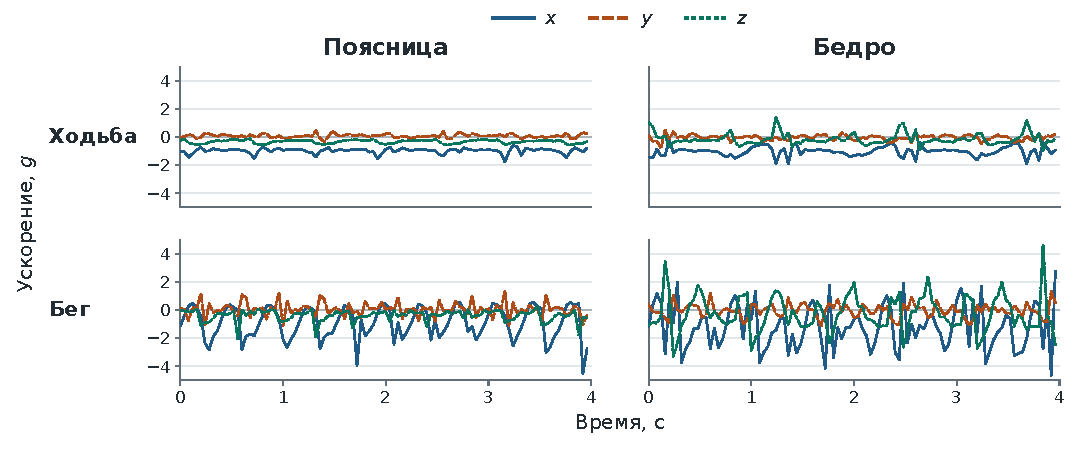
\includegraphics[width=\linewidth,height=6.3cm,keepaspectratio]{harth_walk_run_signals.pdf}
    \par\smallskip
    \small Сигналы акселерометров при ходьбе и беге.
\end{frame}

\begin{frame}{HARTH: графы ходьбы и бега}
    \small Графы (с лагом 2) построенные DIRECTLINGAM. Каждая вершина задана каналом и моментом времени.
    \par\vspace{0.10cm}
    \begin{columns}[T]
        \begin{column}{0.49\textwidth}
            \centering\lead{Ходьба}\par\smallskip
            \timegraph{harth_unrolled_dynotears_walk.png}
        \end{column}
        \begin{column}{0.49\textwidth}
            \centering\lead{Бег}\par\smallskip
            \timegraph{harth_unrolled_dynotears_run.png}
        \end{column}
    \end{columns}
\end{frame}

\begin{frame}{HARTH: сходство внутри и между активностями}
    \begin{columns}[T]
        \begin{column}{0.50\textwidth}
            \small
            \lead{Коэффициент Жаккара}\par\smallskip
            $E_i$ --- множество рёбер графа окна $i$.
            \[
                J(E_i,E_j)=\frac{|E_i\cap E_j|}{|E_i\cup E_j|}.
            \]
            $J=1$ при совпадении, $J=0$ при пустом пересечении.
            \par\smallskip\centering
            \lead{Средний Жаккар по парам окон}\par\smallskip
            \renewcommand{\arraystretch}{1.28}
            \setlength{\tabcolsep}{4pt}
            \begin{tabular}{lcc}
                \toprule
                Метод & \shortstack{Одна\\активность} & \shortstack{Разные\\активности}\\
                \midrule
                DirectLiNGAM & 0.35 & 0.09\\
                PCMCI+ & 0.29 & 0.07\\
                DYNOTEARS & 0.40 & 0.06\\
                \bottomrule
            \end{tabular}
        \end{column}
        \begin{column}{0.46\textwidth}
            \centering\small DYNOTEARS: сходство 16 окон\par\smallskip
            \scalebox{0.95}{\begin{tikzpicture}[x=1cm,y=1cm]
                \node[anchor=north west,inner sep=0] at (0,0) {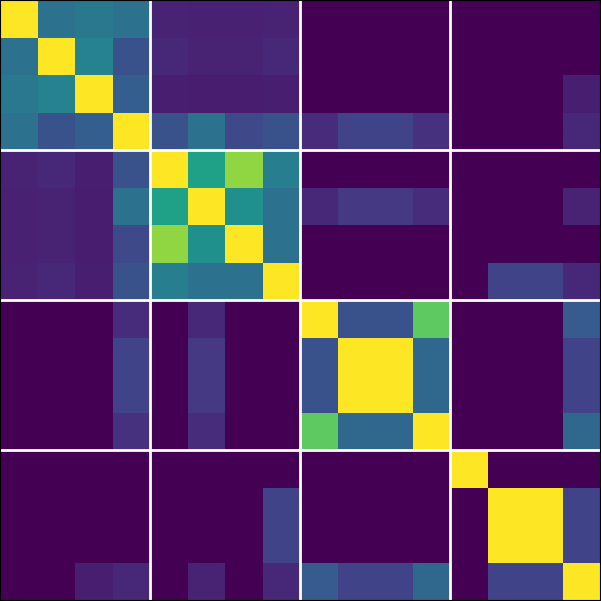
\includegraphics[width=4.65cm]{harth_jaccard_dynotears.png}};
                \foreach \n in {1,4,8,12,16} {
                    \pgfmathsetmacro{\p}{(\n-0.5)*4.65/16}
                    \node[font=\footnotesize,anchor=north] at (\p,-4.70) {\n};
                    \node[font=\footnotesize,anchor=east] at (-0.07,-\p) {\n};
                }
                \node[font=\small] at (2.325,-5.28) {Номер окна $j$};
                \node[font=\small,rotate=90] at (-0.67,-2.325) {Номер окна $i$};
                \node[anchor=south west,inner sep=0] at (4.85,-4.65) {
\includegraphics[width=0.16cm,height=4.65cm]{harth_jaccard_scale.png}};
                \node[font=\footnotesize,anchor=west] at (5.05,0) {1};
                \node[font=\footnotesize,anchor=west] at (5.05,-2.325) {0.5};
                \node[font=\footnotesize,anchor=west] at (5.05,-4.65) {0};
            \end{tikzpicture}}
        \end{column}
    \end{columns}
    \par\smallskip\small Окна 1--4: ходьба; 5--8: бег; 9--12: лестница; 13--16: велосипед.
\end{frame}

\begin{frame}{HARTH: качество классификации}
    \small Рисуем причино-следственные графы используя DIRECTLINGAM (и DYNOTEARS, и PCMCI+), при помощи 1-nn даем метку соотвествующую ближайшему графу.
    \par\medskip
    \centering
    \renewcommand{\arraystretch}{1.28}
    \setlength{\tabcolsep}{7pt}
    \begin{tabular}{lcccc}
        \toprule
        Метод & \shortstack{Верно\\из 140} & Accuracy & \shortstack{Balanced\\accuracy} & Macro $F_1$\\
        \midrule
        DirectLiNGAM + 1-NN      & 126 & 90.0\% & 89.9\% & 89.9\%\\
        \textbf{DYNOTEARS + 1-NN} & \textbf{135} & \textbf{96.4\%} & \textbf{96.2\%} & \textbf{96.4\%}\\
        PCMCI+ + 1-NN        & 118 & 84.3\% & 85.2\% & 84.2\%\\
        Самый частый класс    & 75  & 53.6\% & 50.0\% & 34.9\%\\
        \bottomrule
    \end{tabular}
    \par\medskip\raggedright\normalsize
\end{frame}

\begin{frame}{Текущие результаты}
    \begin{enumerate}
        \item \textbf{Гипотеза оправдалась}
        Действительно для разных процессов причино-следственные графы устроенны по-разному
        \item \textbf{Корректность.} Две леммы объясняют, почему DirectLiNGAM
        восстанавливает граф при выполнении предположений LiNGAM.
        \item \textbf{Классификация HARTH.} DYNOTEARS + 1-NN дают 96.4\% точности.
    \end{enumerate}
\end{frame}

\begin{frame}{Литература и данные}
    \fontsize{8.5}{10}\selectfont
    \begin{enumerate}
        \item Shimizu S. et al. \textit{A Linear Non-Gaussian Acyclic Model for Causal Discovery}. JMLR 7, 2006. \href{https://jmlr.org/papers/v7/shimizu06a.html}{Статья}.
        \item Shimizu S. et al. \textit{DirectLiNGAM: A Direct Method for Learning a Linear Non-Gaussian Structural Equation Model}. JMLR 12, 2011. \href{https://jmlr.org/papers/v12/shimizu11a.html}{Статья}.
        \item Hyvärinen A. et al. \textit{Estimation of a Structural Vector Autoregression Model Using Non-Gaussianity}. JMLR 11, 2010. \href{https://jmlr.org/papers/v11/hyvarinen10a.html}{Статья}.
        \item Zheng X. et al. \textit{DAGs with NO TEARS: Continuous Optimization for Structure Learning}. NeurIPS, 2018. \href{https://arxiv.org/abs/1803.01422}{Статья}.
        \item Pamfil R. et al. \textit{DYNOTEARS: Structure Learning from Time-Series Data}. AISTATS, 2020. \href{https://proceedings.mlr.press/v108/pamfil20a.html}{Статья}.
        \item Runge J. \textit{Causal Network Reconstruction from Time Series: From Theoretical Assumptions to Practical Estimation}. Chaos 28, 2018. \href{https://doi.org/10.1063/1.5025050}{Статья}.
        \item Runge J. \textit{Discovering Contemporaneous and Lagged Causal Relations in Autocorrelated Nonlinear Time Series Datasets}. UAI, 2020. \href{https://proceedings.mlr.press/v124/runge20a.html}{Статья}.
        \item Logacjov A. et al. \textit{HARTH: A Human Activity Recognition Dataset for Machine Learning}. Sensors 21(23), 2021. \href{https://archive.ics.uci.edu/dataset/779/harth}{Данные UCI}.
    \end{enumerate}
\end{frame}

\appendix

\begin{frame}[t]{Дополнение. Почему DirectLiNGAM восстанавливает граф}
    \small
    \setlength{\abovedisplayskip}{3pt}
    \setlength{\belowdisplayskip}{3pt}
    \setlength{\abovedisplayshortskip}{2pt}
    \setlength{\belowdisplayshortskip}{3pt}
    \newcommand{\indep}{\mathrel{\perp\!\!\!\perp}}
    \newcommand{\nindep}{\mathrel{\not\!\perp\!\!\!\perp}}
    \lead{Теорема Дармуа--Скитовича.} Пусть $\varepsilon_k$ взаимно независимы,
    $U=\sum_k a_k\varepsilon_k$ и $V=\sum_k c_k\varepsilon_k$.
    \[
        U\indep V
        \quad\Longrightarrow\quad
        \varepsilon_k \text{ гауссовский для каждого } k
        \text{ с } a_kc_k\ne0.
    \]
    \lead{Лемма 1.}
    $\operatorname{pa}(j)=\varnothing
      \ \Longleftrightarrow\ X_j\indep r_i^{(j)}$ для всех $i\ne j$.
    \[
        \begin{aligned}
        \text{Корень}\qquad &
        X_j=\varepsilon_j,\qquad
        r_i^{(j)}=\sum\nolimits_{k\ne j}d_{ik}\varepsilon_k.\\
        \text{Есть родители}\qquad &
        X_j=\varepsilon_j+\sum\nolimits_{k\ne j}a_{jk}\varepsilon_k,\qquad
        r_i^{(j)}=-\beta_{ij}\varepsilon_j+\sum\nolimits_{k\ne j}d_{ik}\varepsilon_k.
        \end{aligned}
    \]
    Для некоторого родителя $\beta_{ij}\ne0$. По теореме $X_j\nindep r_i^{(j)}$.
    \par\smallskip
    \lead{На выборке.} В статье выбирают узел с минимальным
    $T(j)=\sum_{i\ne j}\widehat I_{\mathrm{ker}}(X_j,r_i^{(j)})$.
    \par
    Взаимную информацию $I$ оценивают по ядерному сходству пар. $I=0$ при независимости.
    \par\smallskip
    \lead{Лемма 2.} Модель для остатков после удаления вклада корня
    \[
        \mathbf r^{(j)}=B_{-j,-j}\mathbf r^{(j)}+\boldsymbol\varepsilon_{-j},
        \qquad \operatorname{pa}(j)=\varnothing.
    \]
    В точном распределении удаление корней даёт порядок, МНК восстанавливает $B$.
    \par\vfill
    Также рассмотрим PCMCI+ и DYNOTEARS (NOTEARS для временных рядов).
\end{frame}

\end{document}
